the approximate solution for $\delta_i\ll 1$ can be expressed introducing an implicit parameteer $\theta$:
  \begin{align}
   r &= \frac{r_m}{2} (1+\cos\theta) \label{eq:r_vs_theta_collapse}\\
   t &= \frac{1}{2H(t_i)}\left(\frac{1+\delta_i}{\delta_i^{3/2}}\right)(\theta-\sin\theta) \label{eq:time_vs_theta_collapse}
  \end{align}
  This evolution is sketched in the left panel of figure \ref{fig:collapse}: every shell starts from a radius $r_i$, expands until it peaks at $r_m$, and then contracts back, finally collapsing to a single point of infinite density at $\theta=2\pi$. 
 
   \begin{figure}
	\centering
	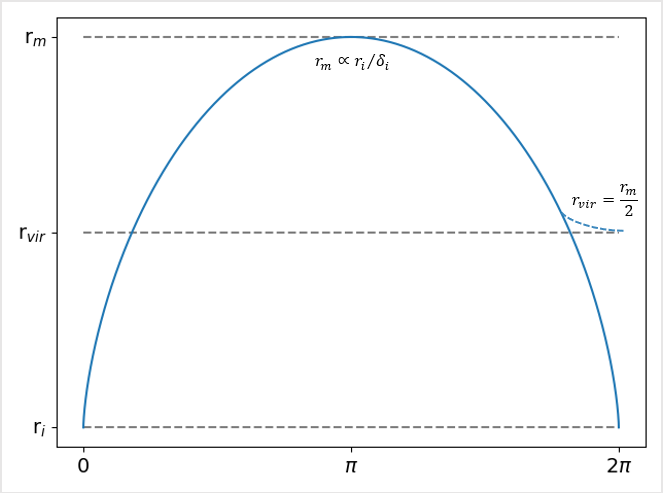
\includegraphics[width=0.45\textwidth]{plots/radius_collapse.PNG}
	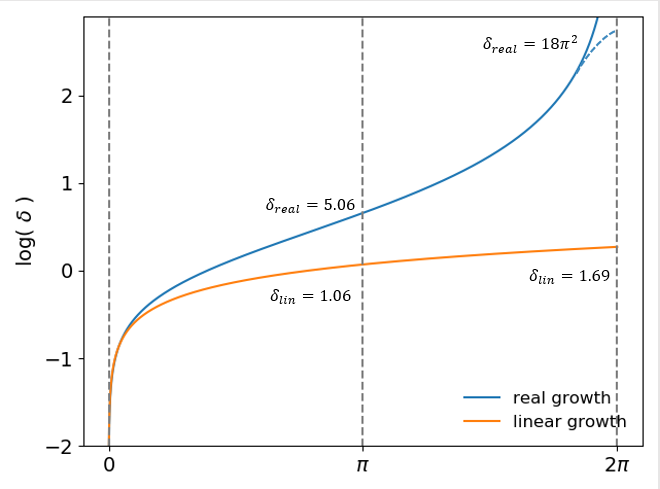
\includegraphics[width=0.45\textwidth]{plots/density_collapse.PNG}
	\caption{\textit{Left panel}: evolution of the radius $r(t)$ for the spherical collapse model according to eqs. \ref{eq:r_vs_theta_collapse},\ref{eq:time_vs_theta_collapse}. The quantities $r_i$, $r_m$, $r_{vir}$ are plotted as grey dashed horizontal lines. The blue dashed line, instead, is a sketch of the radius evolution as the collapse leads to the virialization of the halo. \textit{Right panel}: time evolution of the overdensity $\delta(t)$ according to the same spherical collapse model. The linear growth is plotted as well. Also in this case, the plot shows how virialization prevents the divergence stabilizing the density contrast at the value $\delta_{vir}\approx 18\pi^2$. FIGURE TO BE IMPROVED
	}
	\label{fig:collapse}
    \end{figure}
    
    
      After virialization has taken place, halos have   full density evolution can be obtained analytically , \ref{eq:time_vs_theta_collapse}): it is presented in the right panel of figure \ref{fig:collapse}. Clearly, the overdensity $\delta$ tends to diverge as the collapse proceeds further. The virialization process prevents this divergence: the final overdensity reached by the halos is a constant, and can be determined knowing that the overdensity at $r=r_m$ is $\delta_m = 9\pi^2/16-1$. Since $r_{vir} = r_m/2$, the density of the virialized halo is simply $\rho_{vir}=8\rho_m$. Accounting for the time scaling of the background density, we find:
   \begin{align}
    \delta_{vir} = \frac{\rho_{vir}}{\Bar{\rho}_{vir}}-1 = 32 \frac{
    \rho_m}{\Bar{\rho}_m}-1= 18\pi^2 -1
  \end{align}
  It is interesting to point out that, if we were to follow the linear model and to neglect the non-linear evolution completely, we would find that that, at the time corresponding to collapse, the linear growth of the overdensity would have reached a valued corresponding to $\delta_{lin}\sim 1.69$ (see figure \ref{fig:collapse}). A simplistic interpretation of this result will be very useful in the next section: we can stick to the linear growth model, and consider a halo to be formed whenever the linear overdensity reaches a value greater than $\delta_{lin}\gtrsim 1.69$.
